\chapter{Technische Dokumentation}

\section{Applikationsdokumentation}

\subsection{Diagramme}

\begin{figure}[H]
	\centering
	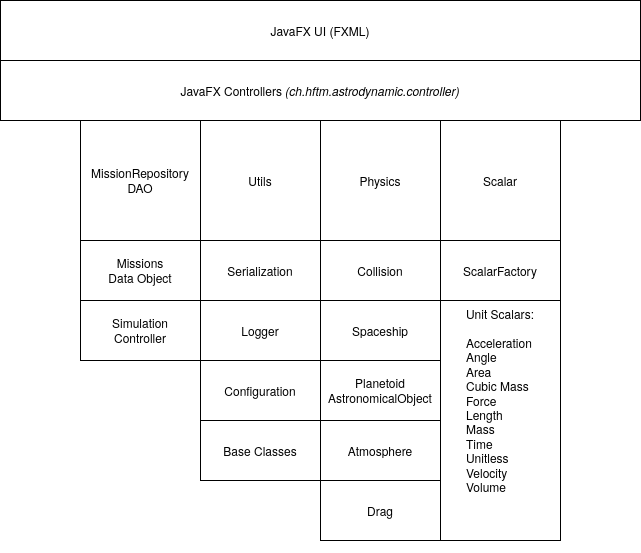
\includegraphics[width=12cm]{res/overview.png}
	\caption{Übersicht Aufbau Astrodynamic}
\end{figure}

\subsection{Maven build}

Um mittels Maven ein Build zu erzeugen kann der Befehl \textit{mvn clean package} verwendet werden.

Dieser Befehl testet das gesamte Softwareprojekt und erzeugt anschliessend im Ordner \textit{target} ein neues Java Executable (JAR File).

\subparagraph{Docker}

Wir haben ebenfalls einen Docker Container vorbereitet, mit welchem das Build automatisiert werden kann.

Dieser nutzt das Zulu OpenJDK, um unser Projekt vollständig zu bauen und zu testen:

\begin{lstlisting}

	# Docker build
	$ docker build -t astrodynamic/build .
	$ docker run --name astrodynamic -v ./:/astrodynamic astrodynamic/build
	# Das Java Executable erscheint im selben Ordner
	
\end{lstlisting}

Mit Docker können wir das Projekt überall mit wenig Aufwand und ohne grossen Installationsaufwand neu bauen.

\section{Themenumsetzung}

\subsection{Unit Tests}

Unsere Unit Tests befinden sich im Ordner \textit{src/test/java/ch/hftm/astrodynamic} und sind nach Anwendungskomponenten gegliedert:

\begin{itemize}
	\item DAO (Data Access Object); Testet den Zugriff und die Fuktionalität des zentrale MissionRepositorys (in welchem alle Missionen und deren Kindobjekte gespeichert sind)
	\item Model; Testet die pedefinierten Modelle (z.B Mond, Erde, Sonne) welche mit der Software mitgeliefert werden
	\item Planetoid; Testet die Funktionalität der Planetoiden (also planetenähnlichen Objekten)
	\item Quad; Testet die Implementation und Abstraktion unseres Quad Datentyps, welcher für alle Berechnungen innerhalb des Projekts verwendet wird
	\item Scalar; Testet die Richtigkeit von Scalar basierten Verrechnungen
	\item SimulationTest; Testet die Simulation der einzelnen Objekte im Sonnensystem
	\item Unit; Testet die verschiedenen Scalar Physik-Einheiten und deren Verrechnungen
	\item Vector; Testet die Vektoren und deren Verrechnungen
\end{itemize}

Wir haben uns primär dafür entschieden, die Business-Logik (primär die Simulation) zu testen, da die Erfolg unseres Projekts primär von der Korrektheit der Simulation abhängig ist.

\subparagraph{Unit Tests ausführen}

Zunächst müssen wir uns ins \textit{astrodynamics} Verzeichnis bewegen in welchem ebenfalls die Datei \textit{pom.xml} gespeichert ist.
Anschliessend können wir die Unit-Tests mit einem einfachen \textit{mvn clean test} ausführen.

\subsection{Enumeration}

Unser wichtigster Einsatz von Enum (Enumeration) findet in der Klasse \textit{Unit} statt. Diese Klasse wird dazu genutzt, SI Einheiten, welche in unserem Projekt verwendet werden, darzustellen:

\begin{lstlisting}
	
	// Contains all physical units as enum
	public enum Unit {
		TIME, // Seconds (s)
		LENGTH, // Meters (m)
		MASS, // Kilogram (kg)
		CURRENT, // Ampere (A)
		TEMPERATURE, // Kelvin (K)
		MOLECULES, // Mol (mol)
		LUNINOSITY, // Candela (cd)
		// Extensions (Implicit)
		VOLUME,  // m ^ 3
		AREA, // m ^ 2
		FORCE, // N
		ACCELERATION, // m/s ^ 2
		VELOCITY, // m/s
		ANGLE, // radian
		ANGULAR_VELOCITY, // radian/second
		ANGULAR_ACCELERATION, // radian/second^2
		// kg ^ 2 imaginary unit for gravitational calculations
		CUBIC_MASS, 
		// kg ^ 2 / m ^ 2 imaginary unit for gravitational calculations
		M2_DIV_L2,
		// N * m ^ 2 * kg ^ 2 gravitational constant
		//  (s ^ -2 * m ^ 3 * kg ^ - 1) 
		F_L2_Mn2,
		// Unitless for scalars without unit
		UNITLESS
	}

\end{lstlisting}

Wir nutzen dieses Enum in allen Skalaren und in diversen Vektoren, um die Einheiten der Werte darzustellen. z.B nutzt die Klasse \textit{LengthScalar}, welche eine Länge speichert, den Wert \textit{LENGTH}.

In den Kommentaren der Klasse werden die genauen Einheiten explizit definiert. Dies hilft bei den Umrechnungen der Werte z.B zwischen verschiedenen Zeiteinheiten (z.B zwischen Stunden, Tagen oder Wochen).

\section{Vererbung}

Wir nutzen Vererbung in allen unseren Klassen. Spezifisch hervorheben möchten wir in diesem Fall die \textit{Scalar} Klassen im Package \textit{ch.hftm.astrodynamic.scalar}, welche allesamt von der Klasse \textit{BaseScalar} im Package \textit{ch.hftm.astrodynamic.utils} erben.

Die einzelnen \textit{Scalar} Klassen stellen jeweils einen spezialisierten Scalar im Projekt dar. z.B werden Längen mittels dem \textit{LengthScalar} dargestellt.
Die Einheiten der jeweiligen Klassen werden in der Kind-Klasse innerhalb des Konstruktors statisch gesetzt und dem Eltern-Konstruktor des \textit{BaseScalar} übergeben und gespeichert.

\section{Casting}

Da wir für die Serialisierung einen eigenen Serializer / Deserializer innerhalb der Klasse \textit{MissionRepository} in \textit{ch.hftm.astrodynamic.utils} implementieren mussten (die Klasse \textit{ObservableList} ist nicht Serialisierbar), verwenden wir Casting in diesem Fall für die Konvertierung zwischen \textit{Object} und \textit{Mission}.

Casting wird ausserdem in einzelnen Fällen innerhalb der Controller verwendet, um z.B einen Double zu einem Integer zu Runden.

\section{Interfaces}

Interfaces werden in unserem Projekt häufig verwendet. Vorwiegend haben wir mittels Interfaces generalisierte Klassen (und deren Vererbungen) implemtiert.

Als Beispiel dient hier das Interface \textit{Scalar} aus dem Package \textit{ch.hftm.astrodynamics.utils}, welches z.B für generalisierte Operationen innerhalb aller Klassen verwendet wird. Mit diesem Interface können wir sicherstellen, dass alle \textit{Scalar} Klassen verglichen oder berechnet werden können.

Ebenfalls ist in diesem Interface eine Implementation für die Funktion \textit{toFittedString()} bereits vorgegeben (und muss aus diesem Grund nicht erneut implementiert werden).

\section{Abstrakte Klassen}

Wir nutzen Abstrakte Klassen unter anderem für unseren \textit{BaseController} im Paket \textit{ch.hftm.astrodynamic.controller} welcher grundlegende Funktionalität für unsere Controller bereitstellt.

Dieser Controller dient als Elternklasse für unsere \textit{Controller} Klassen, wird aber selbst niemals instanziert (daher ist er als Abstract definiert).

Wir verwenden abstrakte Klassen ebenfalls für die \textit{Condition} Klasse für die Mission aus demselben Grund.

\section{Collection}

Der wichtigste Einsatz von Collections in unserem Projekt ist die \textit{ObservableList} innerhalb unseres MissionRepositories.
Dieser Typ der Collection stammt aus dem JavaFX Paket und bietet der Frontend-Anwendung die Möglichkeit, den Inhalt der Liste konstant zu überwachen und Änderungen im UI umgehend darzustellen.


\subparagraph{Sortierung}

Wir sortieren die \textit{ObservableList} innerhalb der Funktion \textit{sort()} innerhalb unserer Klasse \textit{MissionRepository} alphabetisch nach Namen der Mission:


\begin{lstlisting}
	// Sorts the MissionRepository alphabetically
	public static void sort() {
		// Create a comparator for name based sorting 
		Comparator<Mission> byName = (Mission a, Mission b) ->
		a.getName().compareTo(b.getName());
		// Sort the Mission Repository based on names
		getInstance().missions.sort(byName);
	}
\end{lstlisting}

Der Name ist ebenfalls der Primärschlüssel, welcher für die Missionen innerhalb der Funktion \textit{getMissionByName} verwendet wird.

\section{Serialisierung}

Serialisierung wird in unserem Projekt zur Speicherung der Klasse \textit{MissionRepository}, welche den kompletten Status unserer Anwendung enthält verwendet.

Die Klasse \textit{Serializer} ist für die Serialisierung des \textit{MissionRepository} zuständig.
Aktuell wird die Serialisierbarkeit unserer Klassen mittels dem Interface \textit{Serializable} gewährleistet.
Dies ist insbesondere für die Komplexen Datentypen, welche für \textit{Quad} und \textit{ObservableList} verwendet werden, wichtig.
Da \textit{ObservableList} das Interface \textit{Serializable} nicht implementiert, musste im \textit{MissionRepository} mittels der Funktionen \textit{WriteObject()} und \textit{ReadObject()} die Missionen in ein Array konvertiert werden. Dieses Array wird beim Deserialisieren wiederum in Missionen gecasted, welche dem \textit{MissionRepository} hinzugefügt werden.

Ebenfalls wurde eine mögliche Serialisierung ins JSON-Format vorbereitet. Dazu verwenden wir die Bibliothek \textit{Jackson}, welche ebenfalls in diversen Java Web Bibliotheken verwendet wird und als performant gilt.

\section{Speichern und Laden der Missionen}

\subparagraph{Laden}
Beim Start der Anwendung werden die gespeicherten Missionen aus einer Datei geladen.
Der Pfad dieser Datei kann mittels der Konfiguration \textit{STATE FILE} angepasst werden.
Der Standardname der Datei lautet: \textit{state.bin}.
Diese Datei kann ebenfalls gelöscht werden, um den Ursprungszustand wiederherzustellen.

\subparagraph{Speichern}
Wenn Missionen geändert werden, werden diese automatisch in die (aktuell konfigurierte) Projektdatei geschrieben.


\section{Exceptions}

Mit dem \textit{UnitConversionError} im \textit{ch.hftm.astrodynamic.utils} Package haben wir unsere eigene Exception implemementiert.
Diese Exception dient dazu, inkompatible Einheiten in den \textit{Scalar} Klassen abzufangen und zu handeln.
Ebenfalls nutzen wir mit dem \textit{SimulationRuntimeError} eine weitere eigene Exception, welche für Fehler während der Simulation genutzt wird.

\section{Logging}

Wir nutzen unseren eigenen Logger, welchen wir innerhalb der Klasse \textit{Log} in \textit{ch.hftm.astrodynamic.utils} implementiert haben.
Diese Klasse konfiguriert den Logger basierend auf Konfigurationswerten aus der Klasse \textit{ConfigRepository}.
Um den Logger zu nutzen kann die Methode \textit{build()} verwendet werden, welche den konfigurierten Logger des Typs \textit{java.util.logging.Logger} zurückgibt.

\subparagraph{Levels}

Mittels dem Konfigurationswert \textit{LOG LEVEL} kann der Level des Log Outputs definiert werden.
Die Standardkonfiguration für das Level ist auf \textit{INFO} gesetzt. Mit diesem Level werden alle Meldungen mit höherer Priorität als Info ausgegeben. 

\subparagraph{File}

Mittels dem Konfigurationswert \textit{LOG FILE} kann ein Log File definiert werden, in welchen die Logzeilen gespeichert werden.
In der Standardkonfiguration wird das Logfile \textit{astrodynamic.log} verwendet.

\section{Pakete}

Wir strukturieren unser Projekt innerhalb verschiedenen Java Paketen:

\begin{itemize}
	\item controller; Enthält alle Controller für das Frontend
	\item gui; Enthält Komponenten, welche im Frontend verwendet werden
	\item model; Enthält Modelle für die Simulation
	\begin{itemize}
		\item conditions; Enthält Bedingungen für Missionen
		\item planetoids; Enthält vordefinerte Planeten für Missionen
		\item spaceships; Enthält vordefinierte Weltraumfahrzeuge für Missionen
	\end{itemize}
	\item physicts; Enthält Klassen für physikalische Objekte
	\item scalar; Enthält Kinder-Klassen für Scalare (Werte mit zugewiesenen Einheiten)
	\item utils; Enthält Hilfsklassen und Basisklassen
	\item ressources; Enthält Ressourcen (z.B Bilder), welche in unserem Projekt verwendet werden 
\end{itemize}

Diese Pakete können einzeln oder ganz innerhalb des Projekts oder anderen Projekten importiert werden.

\section{Singletons}

Wir nutzen in unserem Projekt Singleton Klassen, um sicherzustellen, dass nur ein einzelnes statisches Element veränderbar ist.

Ein Beispiel einer solchen Klasse ist das \textit{MissionRepository} aus dem Paket \textit{ch.hftm.astrodynamic.utils}.
Die integrierte \textit{ObservabeList missions} muss für das gesamte Projekt während der Laufzeit einmalig sein. Damit wir keine Instanzen übergeben müssen, instanzieren wir diese Liste statisch.

Während die Liste selbst statisch bleibt, kann das MissionRepository jederzeit instanziert werden.
